\documentclass[12pt]{article}

%------------ Packages -----------
\usepackage[margin=1in]{geometry}
\usepackage{enumitem}
%set margins to 1 inch
\usepackage{amsmath}
\usepackage{amssymb}
\usepackage{amsfonts}
\usepackage{amsthm}  % AMS theorem environments and proof environment -- load after amsmath
\renewcommand\qedsymbol{$\blacksquare$}
\usepackage{latexsym}
\usepackage{graphicx}    % standard LaTeX graphics tool
\usepackage{xypic}      % commutative diagrams
\usepackage{tikz}
\usepackage{cancel}
\usepackage{hyperref}
\hypersetup{
        colorlinks,
        citecolor=black,
        filecolor=black,
        linkcolor=black,
        urlcolor=black
}
\usepackage{float}

%------------- Headers -----------

\usepackage{fancyhdr}
\pagestyle{fancy}
\lhead{MATH 273 Definitions and Theorems}
\rhead{December 5 2020}
\chead{}
%\lfoot{Author's Name}
%\cfoot{}
%\rfoot{Page \thepage}


%------------- Environments -------

\newtheorem{thm}{Theorem}[section]
\newtheorem*{thm*}{Theorem}
\newtheorem{lem}[thm]{Lemma}  %%%% [thm] means number in sequence with Theorem
\newtheorem{cor}[thm]{Corollary}
\newtheorem{prop}[thm]{Proposition}
\newtheorem{axi}[thm]{Axiom}
%%% definition style
\theoremstyle{definition}
\newtheorem{defn}[thm]{Definition}
\newtheorem{eg}[thm]{Example}
\newtheorem{xca}[thm]{Exercise}
\newtheorem{conj}[thm]{Conjecture}
%%% remark style
\theoremstyle{remark}
\newtheorem{rmk}[thm]{Remark}
\newtheorem*{qst}{Question}
\newtheorem{obs}[thm]{Observation}
\newtheorem*{note}{Note} %%%%%%%%%% no numbering for notes
\numberwithin{equation}{section}

%------------- Macros -------------
\newcommand{\ip}[2]{\langle #1 , #2 \rangle}    %this is to get the correct brackets for inner product
\newcommand{\abs}[1]{\lvert#1\rvert}
\newcommand\diag{\operatorname{diag}}   %%%%%%%%% diag matrix
\newcommand\tr{\mbox{tr}\,}   %%%%%%%%% trace
\newcommand\C{\mathbb C}    %%%%%%%%% the set of complex numbers
\newcommand\R{\mathbb R}    %%%%%%%%% the set of real numbers
\newcommand\Z{\mathbb Z}    %%%%%%%%% the set of integers
\newcommand\N{\mathbb N}    %%%%%%%%% the natural numbers
\newcommand\Q{\mathbb Q}    %%%%%%%% the rational numbers
%% math operators
\DeclareMathOperator{\ran}{Im} %% image
\DeclareMathOperator{\aut}{Aut} %% automorphism
\DeclareMathOperator{\spn}{span} %% span
\DeclareMathOperator{\ann}{Ann} %% annihilator 
\DeclareMathOperator{\rank}{rank} %% rank
\DeclareMathOperator{\ch}{char}        %% characteristic
\DeclareMathOperator{\ev}{\bf{ev}}    %% evaluation
\DeclareMathOperator{\sgn}{sgn} %% sign
\DeclareMathOperator{\id}{Id} %% identity
\DeclareMathOperator{\supp}{Supp}%%%%%%%% support


%------------- Begin --------------

\begin{document}

%%%%%%%%%%%%%%%%%%%%%%%%%%%%%%%%%%

\title{Math 273 Definitions and Theorems}
\author{E/Ea Thompson(they/them)}
\maketitle

\tableofcontents

%%%%%%%%%%%%%%%%%%%%%%%%%%%%%%%%%%


\section{Integers and Division}

\subsection{Definitions}


\begin{defn}[Parity]
        An integer $n \in \Z$ is even if and only if there exists $l \in \Z$ so that $n = 2l$. An integer $n \in \Z$ is odd if and only if there exists $l \in \Z$ so that $n = 2l + 1$
\end{defn}

\begin{defn}[Divisibility]
        Let $a,b \in \Z$.
        a divides b, $a\;\vert\;b$, $\iff$ there exists $k \in \Z$ so that $b = ak$
\end{defn}


\begin{defn}[GCD]
        Let $a,b \in \Z$, not both zero. The \textbf{greatest common divisor} of a and b, denoted $\gcd(a,b)$, is the unique integer d with the following properties:
        \begin{enumerate}
                \item $d\;\vert\;a$ and $d\;\vert\;b$
                \item For all $c \in \Z$, if $c\;\vert\;a$ and $c\;\vert\;b$, then $c \leq d$.
        \end{enumerate}
\end{defn}


\begin{defn}[Relatively Prime]
        Let $a,b \in \Z$. Then a and b are relatively prime $\iff$ $\gcd(a,b) = 1$.
\end{defn}


\begin{defn}[Prime]
        An integer n is prime $\iff$ $n > 1$ and for all $r,s \in \N$, if $n = rs$ then either $r = 1$ and $s = n$ or $r = n$ and $s= 1$. On the other hand, n is composite $\iff$ $n > 1$ and there exist $r,s \in \N$ so that $n = rs$ and $1 < r,s < n$.
\end{defn}





\subsection{Theorems}


\begin{thm*}[1]
        For all integers a and b, if a and b are positive and a divides b, then a is less than b or a is equal to b.
\end{thm*}
\begin{proof}
        Suppose $a,b \in \Z$. Further suppose $a,b > 0$ and $a\;\vert\;b$. Then there exists $k \in \Z$ so that $ak = b$. Then since $a > 0$ and $ak = b > 0$, it follows that $k > 0$. Moreover, since $k \in \Z$ and $k > 0$, it follows that $$1 \leq k$$ Thus, by multiplying both sides by a we find that $a \leq ak = b$, as claimed.         
\end{proof}




\begin{thm*}[2]
        For all $a,b,c \in \Z$, if $a\;\vert\;b$ and $b\;\vert\;c$, then $a\;\vert\;c$.
\end{thm*}


\begin{axi}[Well-Ordering Principle]
        For any non-empty subset S of $\N$, there exists a least element $s \in S$ such that for all $x \in S$, $s \leq x$.
\end{axi}


\begin{thm*}[Quotient-Remainder]
        For all $n \in \Z$ and $d \in \N$ there exists unique integers q and r such that $n = dq + r$ and $0 \leq r < d$.
\end{thm*}




\begin{lem}[Squares]
        For all $n \in \Z$, if 2 divides $n^2$ then 2 divides n.
\end{lem}


\begin{lem}[gcd-lemma]
        Let $a,b \in \Z$ not both zero. For any $q,r \in \Z$, if $a = qb + r$ then $\gcd(a,b) = \gcd(b,r)$.
\end{lem}


\begin{thm*}[Baezue's Identity]
        For any $a,b \in \Z$ not both zero, there exists $x,y \in \Z$ so that $\gcd(a,b) = ax + by$, and $\gcd(a,b)$ is the smallest positive integer that can be written in the form $ax + by$, $x,y \in \Z$.
\end{thm*}



\begin{cor}
        For all $a,b \in \Z$, a and b are relatively prime if and only if there exist $x,y \in \Z$ so that $xa + yb = 1$.
\end{cor}



\begin{lem}[4]
        Let $p \in \Z$ be a prime. For any $a \in \Z$, if $p\;\vert\;a$, then $p\;\cancel{\vert}\;(a+1)$.
\end{lem}


\begin{lem}[5]
        For all $n\in \N$, $n > 1$, there exists a prime p such that $p \;\vert\;n$.
\end{lem}

\begin{thm*}[6]
        There are infinitely many prime numbers.
\end{thm*}



\begin{thm*}[Fundamental Theorem of Arithmetic]
        Given any integer $n$, $n >1$, there exists a positive integer k, distinct primes $p_1,p_2,...,p_k$, and positive integers $e_1,e_2,...,e_k$ such that $$n = p_1^{e_1}p_2^{e_2}...p_k^{e_k},$$ and any other expansion for n as a product of prime numbers is identical to this one, except for possible reordering the prime factors.
\end{thm*}



\begin{thm*}[Prime or Composite]
        For any natural number $n$, if $n > 1$ then $n$ is either prime or composite.
\end{thm*}



\begin{thm*}[Integral Combinations]
        All integral combinations of natural numbers $a$ and $b$ are multiples of $\gcd(a,b)$.
\end{thm*}




\clearpage

\section{Modolar Arithmetic}


\subsection{Definitions}


\begin{defn}[Congruence modulo d]
        Let $d \in \N$, $d >1$. For any $a,b \in \Z$, if $d\;\vert\;a-b$, then we say that ``a is congruent to b modulo d" and we write $a \equiv b \mod d$
\end{defn}


\begin{note}
        If $d\;\cancel{\vert}\;a-b$, then we write $a \cancel{\equiv}b\mod d$.
\end{note}



\begin{defn}
        For all $d \in \N$, $d >1$, and for all $a,b \in \Z$, define 
        \begin{equation}
                \begin{array}{c}
                        [a]_d+[b]_d=[a+b]_d \\
                        {}[a]_d[b]_d = [ab]_d
                \end{array}
        \end{equation}
\end{defn}




\subsection{Theorems}


\begin{lem}[7]
        For all $d \in \N$, $d > 1$, and for all $n \in \Z$, n is congruent to one of $0,1,...,d-1$ modulo d.
\end{lem}


\begin{lem}[8]
        For all $d \in \N$, $d > 1$, and for all $a,b,r,s \in \Z$, if $a \equiv b\mod d$ and $r \equiv s \mod d$, then $a + r\equiv b + s\mod d$ and $ar\equiv bs \mod d$.
\end{lem}

\begin{note}
        $\Z/d\Z = \{[a]_d:a \in \Z\}$, where $[a]_d = \{b \in \Z: b \equiv a \mod d\}$.
\end{note}


\begin{cor}
        For all $d \in \N$, $d > 1$, and for all $a\in \Z$, if $\gcd(a,d) = 1$, then there exists an integer s so that $as \equiv 1 \mod d$. In this case, $[s]_d = [a]_d^{-1}$ is the multiplicative inverse of a modulo d. 
\end{cor}


\begin{thm*}[Euclid's Lemma]
        For all $a,b,c \in \Z$, if $\gcd(a,c) = 1$ and $a\;\vert\;bc$, then $a\;\vert\;b$
\end{thm*}

\begin{cor}[10]
        For all $a,b,c,d \in \Z$, where $d > 1$, if $\gcd(c,d) = 1$ and $ac \equiv bc \mod d$ then $a \equiv b \mod d$.
\end{cor}


\begin{thm*}[Fermat's Little Theorem]
        If p is prime, then for any $a \in \Z$ such that $p\;\cancel{\vert}\;a$ and $$a^{p-1}\equiv 1 \mod p$$
\end{thm*}



\begin{thm*}[Chinese Remainder Theorem]
        Suppose that $n_1,n_2,...,n_k \in \N$ are pairwise relatively prime (i.e. $\gcd(n_i,n_j) = 1$ for all $1 \leq i \neq j \leq k$) For all $a_1,a_2,...,a_k \in \Z$, the system of congruences 
        \begin{equation}
                \left\{\begin{array}{c}
                        x \equiv a_1 \mod n_1 \\
                        x \equiv a_2 \mod n_2 \\
                        \vdots \\
                        x \equiv a_k \mod n_k
                \end{array}\right.
        \end{equation}
        has a unique solution modulo $N = n_1n_2...n_k$.
\end{thm*}



\clearpage


\section{Sets}


\subsection{Definitions}


\begin{defn}[Set]
        \begin{enumerate}
                \item A set is a well-defined collection of objects 
                \item The objects that make up the set are called elements
        \end{enumerate}
\end{defn}


\begin{defn}[Subset]
        A is a subset of B, written $A \subset B$ $\iff$ for all $x \in A$, $x \in B$.
\end{defn}


\begin{defn}[Proper Subset]
        A is a proper subset of B, written $A \subsetneq B$ $\iff$ $A \subset B$ and there exists $x \in B$ such that $x \notin A$.
\end{defn}



\begin{defn}[Equality]
        Let A and B be sets. Then $A = B$ $\iff$ $A \subset B$ and $B \subset A$.
\end{defn}



\begin{defn}[Cartesian Product]
        The \textbf{Cartesian Product} of sets A and B, denoted $A \times B$ is the set $\{(a,b): a\in A\;\text{and}\; b \in B\}$ of ordered pairs of elements in A and B.
\end{defn}




\subsection{Theorems}


\begin{lem}[12]
        For every set X, the empty set $\emptyset$ is a subset of X.
\end{lem}


\begin{thm*}[13] Let A, B, and C be sets.
        \begin{enumerate}
                \item $A \cap B \subset A$ and $A \cap B \subset B$
                \item $A \subset A \cup B$ and $B \subset A \cup B$
                \item If $A \subset B$ and $B \subset C$, then $A \subset C$
        \end{enumerate}
\end{thm*}



\begin{lem}[14]
        For any sets A and B, if $A \subset B$, then $A \cap B = A$ and $A\cup B = B$.
\end{lem}



\begin{lem}[15]
        There is only one set with no elements.
\end{lem}



\begin{prop}[16]
        For all sets A, B, and C, if $A \subset B$ and $B \subset C^c$, then $A\cap B = \emptyset$.
\end{prop}


\clearpage


\section{Functions}


\subsection{Definitions}


\begin{defn}[Function]
        A function from a set A to a set B is a subset f of $A \times B$ so that for all $x \in A$ there exists a unique $y \in B$ so that $(x,y) \in f$.
        \begin{enumerate}
                \item A is the \textbf{domain} of f
                \item B is the \textbf{codomain} of f
                \item If $(x,y) \in f$ we say that $y$ is the image of $x$ under f, and we write $f(x)=y$
        \end{enumerate}
\end{defn}



\begin{defn}[Composition]
        Let $f:A \rightarrow B$ and $g: B \rightarrow C$ be functions. The composition of g and f, or the composite of g and f, is the function $g \circ f: A \rightarrow C$ given by $(g\circ f)(x) = g(f(x))$ for all $x \in A$
\end{defn}


\begin{defn}[Bijectivity] Let $f:A\rightarrow B$ be a function.
        \begin{enumerate}
                \item f is injective $\iff$ for all $a,a' \in A$, if $f(a) = f(a')$ then $a = a'$
                \item f is surjective $\iff$ for all $b \in B$ there exists $a \in A$ so that $f(a) = b$
                \item f is bijective $\iff$ it is both injective and surjective
        \end{enumerate}
\end{defn}


\begin{defn}[Identity]
        The identity function (on X) is the function $I_X:X \rightarrow X$ given by $I_X(x) = x$ for all $x \in X$
\end{defn}


\begin{note}
        The identity function is a bijection.
\end{note}



\begin{defn}
        A function $g:B \rightarrow A$ is an inverse of $f:A \rightarrow B$ $\iff$ $g\circ f = I_A$ and $f\circ g= I_B$.
\end{defn}



\begin{defn}[Cardinality]
        Let A and B be two sets. A and B have the same \textbf{cardinality}, written $|A| = |B|$, $\iff$ there exists a bijection $f:A\rightarrow B$. A is said to be finite $\iff$ there exists $n \in \N$ so that $|A| = |\{1,...,n\}|$
\end{defn}


\begin{defn}[Countable]
        Let A be an infinite set. A is countable $\iff$ $|A| = |\N|$. A is uncountable $\iff$ A is not countable.
\end{defn}



\begin{defn}[Image]
        Let $f:A \rightarrow B$ be a function, the image of f is the set $$\text{Im}(f) := \{b \in B: \exists a \in A, f(a) = b\}$$
\end{defn}


\begin{defn}[Boundedness]
        Let $S \subset \R$. We say that S is bounded if and only if there exists $M \in \R$ so that for all $x \in S$, $|x| < M$. Otherwise, S is unbounded
\end{defn}


\begin{defn}
        Let $f:\R \rightarrow \R$ be a function. Let $A \subset \R$.
        \begin{enumerate}
                \item $f$ is strictly increasing on A $\iff$ for all $a,b \in A$ if $a<b$ then $f(a) < f(b)$
                \item $f$ is strictly decreasing on A $\iff$ for all $a,b \in A$ if $a < b$ then $f(a) > f(b)$
                \item $f$ is non-decreasing on A $\iff$ for all $a,b \in A$ if $a < b$ then $f(a) \leq f(b)$
                \item $f$ is non-increasing on A $\iff$ for all $a,b \in A$ if $a < b$ then $f(a) \geq f(b)$
                \item $f$ is monotone on A $\iff$ $f$ is non-decreasing on A or $f$ is non-increasing on A
                \item $f$ is strictly monotone on A $\iff$ $f$ is increasing on A or $f$ is decreasing on A
                \item $f$ is bounded on A $\iff$ $\text{Im}(f)$ is a bounded subset of $\R$
                \item $f$ is unbounded on A $\iff$ $\text{Im}(f)$ is not bounded on A.
        \end{enumerate}
\end{defn}






\subsection{Theorems}


\begin{lem}[17]
        A function $f:A \rightarrow B$ is a bijection $\iff$ f has a two-sided inverse.
\end{lem}



\begin{lem}[18]
        If $f:A \rightarrow B$ is a bijection, then the inverse function is unique and we denote it by $f^{-1}:B\rightarrow A$.
\end{lem}


\begin{cor}[19]
        If $f:A \rightarrow B$ is a bijection, then $f^{-1}:B \rightarrow A$ is a bijection with inverse $f$.
\end{cor}


\begin{prop}[20]
        $\Z$ is countable.
\end{prop}




\begin{thm*}[Composition]
        The composition of two surjections is a surjection and the composition of two injections is an injection.
\end{thm*}



\begin{thm*}[Unions of Countable Sets]
        For any $n \in \N$, if $\mathcal{A} = \{A_1,...,A_n\}$ is a collection of countable sets, then \begin{equation}
                \bigcup\limits_{A_i \in \mathcal{A}} A_i
        \end{equation}
        is also countable.
\end{thm*}




\begin{thm*}[Inverses]
        Let $f:A \rightarrow B$ be a function. If $f$ has a left-sided inverse then $f$ is injective, and if $f$ has a right-sided inverse then $f$ is surjective.
\end{thm*}




\begin{thm*}[Equivalent Definitions of Countable]
        Let A be an infinite set. Then A is countable if and only if 
        \begin{enumerate}
                \item there exists an injection $f:A\rightarrow \N$
                \item there exists a surjection $g:\N\rightarrow A$
        \end{enumerate}
\end{thm*}




\clearpage


\section{Relations}



\subsection{Definitions}

\begin{defn}[Relation]
        Let A be a set. A (binary) relation on a set A is a subset of $A \times A$.
\end{defn}

\begin{defn}[Properties]
        Let R be a relation on A.
        \begin{enumerate}
                \item R is \textbf{reflexive} $\iff$ for all $x \in A$, $x\;R\;x$
                \item R is \textbf{symmetric} $\iff$ for all $x,y \in A$, if $x\;R\;y$ then $y\;R\;x$
                \item R is \textbf{transitive} $\iff$ for all $x,y, z \in A$, if $x\;R\;y$ and $y\;R\;z$ then $x\;R\;z$
        \end{enumerate}
\end{defn}



\begin{defn}[Equivalence Relation]
        Let R be a relation on a set A. Then R is an equivalence relation $\iff$ R is reflexive, symmetric, and transitive.
\end{defn}


\subsection{Theorems}

\begin{lem}[21]
        Let A be a set. Let R be an equivalence relation on A. Define $[a]=\{b \in A: a\;R\;b\}$ to be the equivalence class of $a \in A$. The set A is the disjoint union of distinct equivalence classes.
\end{lem}



\begin{thm*}[21]
        Let $n \in \Z$, $n > 1$. The relation congruence modulo n is an equivalence relation on $\Z$ with distinct equivalence classes $[0],[1],...,[n-1]$.
\end{thm*}



\section{Construction of $\Z$ and $\Q$}



\subsection{Definitions}

\begin{defn}[Relation on $\N \times \N$]
        Define a relation $\sim$ on $\N \times \N$ as follows: $$\forall (a,b),(c,d) \in \N\times \N, (a,b)\sim(c,d) \iff a + d = c + b$$
\end{defn}


\begin{defn}[Integers]
        $\Z := \N\times\N/\sim = \{[(a,b)]:a,b \in \N\}$ to be the set of equivalence classes of $\sim$ on $\N\times\N$.
\end{defn}


\begin{defn}[Integer Operations]
        For all $[(a,b)],[(c,d)] \in \Z$, we define operations $+$ and $\times$ by: $$[(a,b)]+[(c,d)] = [(a+c,b+d)]$$ and $$[(a,b)]\times[(c,d)] = [(ac+bd,ad+bc)]$$
\end{defn}


\begin{defn}[Relations on $\Z \times \Z^*$]
        We define the relation $\approx$ on $\Z \times \Z^*$ by for all $(a,b),(c,d) \in \Z\times\Z^*$, $(a,b)\approx(c,d)$ $\iff$ $ad = bc$.
\end{defn}



\begin{defn}[$\Q$]
        The rational numbers $\Q$ are defined to be the equivalence classes for the relation $\approx$ $$\Q := \Z\times\Z^*/\approx = \{[(a,b)]:(a,b) \in \Z\times\Z^*\}$$ We identify $(a,b)$ with $\frac{a}{b}$
\end{defn}


\begin{defn}[Rational Operations]
        For all $[(a,b)],[(c,d)]\in \Q$ we define operations $+$ and $\times$ by: $$[(a,b)] + [(c,d)] = [(ad + bc,bd)]$$ and $$[(a,b)]\times[(c,d)] = [(ac,bd)]$$
\end{defn}


\begin{defn}[Lowest Terms]
        A rational number $\frac{a}{b} \in \Q$ is in lowest terms $\iff$ $b > 0$ and $\gcd(a,b) = 1$.
\end{defn}



\begin{defn}[Irrational]
        Let $x \in \R$ be a real number, then x is irrational $\iff$ $x \notin \Q$.
\end{defn}







\subsection{Theorems}


\begin{prop}[22]
        The relation $\sim$ on $\N\times \N$ is an equivalence relation.
\end{prop}


\begin{thm*}[23]
        The operations defined on $\Z$ form a commutative ring with identity (in particular $\Z$ is an integral domain).
\end{thm*}


\begin{lem}[24]
        For any $n \in \Z$, $0n = 0$.
\end{lem}


\begin{lem}[25]
        For any $a \in \Z$, the additive inverse $-a$ is unique and $-a = (-1)a$.
\end{lem}


\begin{prop}[26]
        The relation $\approx$ $\Z\times\Z^*$ is an equivalence relation.
\end{prop}



\begin{thm*}[27]
        The operations on $\Q$ define a field.
\end{thm*}



\begin{lem}[28]
        For all $q \in \Q$, $q = \frac{a}{b}$ is in lowest terms if and only if b is the smallest positive integer such that $q = \frac{a}{b}$
\end{lem}



\begin{lem}[29]
        The real numbers are the disjoint union of the rational numbers and the irrational numbers.
\end{lem}



\begin{thm*}[Irrationality of $\sqrt{2}$]
        The square root of 2 is irrational.
\end{thm*}


\begin{cor}[Irrational Prime Roots]
        For all $p \in \N$, if p is a prime then $\sqrt{p} \notin \Q$.
\end{cor}



\clearpage


\section{Sequences in $\Q$}



\subsection{Definitions}

\begin{defn}[Sequence]
        A sequence in a set A is a function $a:\N \rightarrow A$. By convention we write $a_n = a(n)$ for all $n \in \N$, and we write $a:\N \rightarrow A$ as $\{a_n\} = \{a_n\}_{n=1}^{\infty}$.
\end{defn}


\begin{rmk}[Order on $\Q$]
        On $\N$ we have a notion of $<$ that we can transport to $\Q$ to get an ordering on $\Q$ and $$\Q^+ := \{q \in \Q: q > 0\}$$
\end{rmk}


\begin{defn}[Convergence]
        Let $\{a_n\}$ be a sequence of rational numbers. The sequence $\{a_n\}$ converges to a limit $L \in \Q$ $\iff$ for all $\frac{1}{M} \in \Q$, $\frac{1}{M} > 0$, there exists $N \in \N$ so that for all $n \in \N$, if $n \geq N$ then $|a_n - L| < \frac{1}{M}$. If $\{a_n\}$ converges and has limit L, we write $a_n\rightarrow L$. If $\{a_n\}$ does not converge we say it diverges.
\end{defn}



\begin{defn}[Cauchy Sequences in $\Q$]
        Let $\{a_n\}_{n=1}^{\infty}$ be a sequence in $\Q$. $\{a_n\}_{n=1}^{\infty}$ is Cauchy $\iff$ for all $\frac{1}{M} \in \Q$, $\frac{1}{M} > 0$, there exists $N \in \N$ so that for all $m,n \in \N$, if $m,n \geq N$ then $|a_n - a_m| < \frac{1}{M}$.
\end{defn}








\subsection{Theorems}

\begin{lem}[32 Triangle Inequality]
        For all $a,b \in \Q$, $|a+b| \leq |a| + |b|$.
\end{lem}


\begin{lem}[33]
        If $\{a_n\}\subset \Q$ converges to $L \in \Q$, then $\{a_n\}$ is Cauchy.
\end{lem}



\begin{thm*}[Countability]
        The rational numbers are countable.
\end{thm*}

\clearpage


\section{Constructing $\R$}



\subsection{Definitions}


\begin{defn}[Binary Operations]
        Let S be a set. A binary operation on S is a function $*:S\times S \rightarrow S$. For all $x,y \in S$, we usually denote $*((x,y))$ by $x*y$
        \begin{enumerate}
                \item The binary operation $*$ on S is commutative $\iff$ for all $x,y \in S$ $x*y=y*x$
                \item The binary operation $*$ on S is associative $\iff$ for all $x,y,z\in S$, $(x*y)*z=x*(y*z)$
                \item An element $e \in S$ is an identity element for $*$ $\iff$ for all $x \in S$ $x*e = e*x = x$.
        \end{enumerate}
\end{defn}


\begin{defn}[Field]
        A field is a triple $(F,+,*)$ consisting of a set F and two binary operations which form abelian groups over F and for all $a,b,c \in F$, $$a(b+c) = ab+ac$$
\end{defn}



\begin{defn}[Order Axioms]
        A positive set in a field F is a subset $P \subset F$ such that 
        \begin{enumerate}
                \item $\forall x,y \in P, x+y \in P$
                \item $\forall x,y \in P, xy \in P$
                \item $\forall x \in F$, exactly one of: $x = 0$, $x \in P$ or $-x \in P$ is true (Trichotomy Property).
        \end{enumerate}
        Define $\forall x,y \in F, x < y \iff y-x \in P$
\end{defn}



\begin{defn}[Relation on $\mathcal{S}$]
        For all $\{a_n\},\{b_n\} \in \mathcal{S}$, $\{a_n\}\sim\{b_n\}$ $\iff$ $\{a_n\} - \{b_n\}$ converges to 0.
\end{defn}


\begin{defn}[Real Numbers]
        The real numbers $\R$ are defined to be the set $$\R:= \mathcal{S}/\sim = \{[\{a_n\}]:\{a_n\}\in\mathcal{S}\}$$ of equivalence classes on $\mathcal{S}$ under the equivalence relation $\sim$
\end{defn}




\begin{defn}[Positive Reals]
        The real number $\alpha \in \R$ is positive $\iff$ for all $\{a_n\} \in \alpha$, there exist $k,N \in \N$ so that if $n \geq N$, then $a_n > \frac{1}{k}$. The real number $\alpha \in \R$ is positive $\iff$ $-\alpha = [\{-a_n\}:\{a_n\} \in \alpha]$ is positive.
\end{defn}


\begin{defn}[Operations on $\R$]
        Let $\alpha,\beta \in \R$. Choose representatives $\{a_n\} \in \alpha$, $\{b_n\} \in \beta$. Then $\alpha + \beta = [\{a_n+b_n\}]$ and $\alpha\beta=[\{a_nb_n\}]$
\end{defn}




\subsection{Theorems}


\begin{lem}[35]
        Let $\mathcal{S}$ be the set of Cauchy sequences of rational numbers. For all $\{a_n\},\{b_n\} \in \mathcal{S}$ and $c \in \Q$.
        \begin{enumerate}
                \item $\{a_n\}+\{b_n\} = \{a_n+b_n\}\in \mathcal{S}$
                \item $\{a_n\}\{b_n\} = \{a_nb_n\} \in \mathcal{S}$
                \item $c\{a_n\} = \{ca_n\} \in \mathcal{S}$
        \end{enumerate}
\end{lem}


\begin{prop}[36]
        The relation $\sim$ on $\mathcal{S}$ is an equivalence relation.
\end{prop}



\begin{prop}[37]
        Addition and multiplication on $\R$ is well-defined.
\end{prop}



\begin{lem}[38]
        If a Cauchy sequence $\{a_n\} \in \mathcal{S}$ has a convergent subsequence $\{a_{n_j}\}_{j=1}^{\infty}$, $n_j \in \N$, then $\{a_n\}$ converges to the same limit.
\end{lem}



\begin{lem}[39]
        For all Cauchy sequences $\{a_n\},\{b_n\} \in \mathcal{S}$
        \begin{enumerate}
                \item If $a_n \rightarrow 0$ and $b_n \rightarrow 0$, then $\{a_n + b_n\}$ converges to 0.
                \item If $a_n \rightarrow 0$, then $\{a_nb_n\}$ converges to 0.
        \end{enumerate}
\end{lem}

\clearpage


\section{Properties on $\R$}



\subsection{Definitions}

\begin{defn}[Completeness]
        An ordered field F is complete $\iff$ for all sequences $\{a_n\} \subset F$, if $\{a_n\}$ is cauchy then $\{a_n\}$ converges.
\end{defn}


\begin{defn}[Upper Bound]
        If $S \subset F$ is a subset, then $\beta \in F$ is an upper bound for S if for all $x \in S$ $x \leq \beta$. An upper bound $\beta$ for S is a least upper bound of S $\iff$ for all upper bounds $\beta'$ of S, $\beta \leq \beta'$
\end{defn}



\begin{defn}[Archimedean Property]
        For all $x,y \in \R$, if $x > 0$ then there exists $n \in \N$ so that $nx > y$
\end{defn}



\begin{defn}[Infimums and Supremums]
        Suppose that $S \subset \R$ that is bounded. Then the greatest lower bound of $S$ is called the infimum of $S$, and denoted $\inf(S)$. Equivalently, the least upper bound of $S$ is called the supremum of $S$, and denoted $\sup(S)$.
\end{defn}




\subsection{Theorems}


\begin{lem}[Lemma X]
        An ordered field F is complete and has the Archimedean property $\iff$ for every nonempty subset $U \subset F$, if $U$ has an upper bound in F, then $U$ has a least upper bound on F.
\end{lem}



\begin{thm*}[$\R$ has the Least Upper Bound Property]
        For every nonempty subset $U$ of $\R$, if $U$ has an upper bound then $U$ has a least upper bound.
\end{thm*}



\begin{cor}[41 Existence of Root 2]
        The square root of 2 is a real number.
\end{cor}


\begin{thm*}[42 Archimedean Property of $\R$]
        For all $x,y \in \R$, if $x > 0$, then there exists $n \in \N$ so that $nx >y$.
\end{thm*}



\begin{cor}[43]
        The Archimedean property of $\R$ is equivalent to the following statement:$$\forall \varepsilon \in \R, \varepsilon > 0, \exists n \in \N: 0 < \frac{1}{n} < \varepsilon$$
\end{cor}



\begin{thm*}[Sup and Inf]
        The Greatest Lower Bound property is equivalent to the Least Upper Bound property.
\end{thm*}



\clearpage


\section{Sequences in $\R$}



\subsection{Definitions}

\begin{defn}[Sequences]
        Let $\{a_n\}$ be a sequence of real numbers.
        \begin{enumerate}
                \item $\{a_n\}$ converges to $L \in \R$ $\iff$ for all $\varepsilon \in \R$, $\varepsilon > 0$, there exists $N \in \N$ so that for all $n \in \N$, if $n \geq N$ then $|a_n - L| < \varepsilon$
                \item $\{a_n\}$ is Cauchy $\iff$ for all $\varepsilon \in \R$, $\varepsilon > 0$, there exists $N \in \N$ so that for all $m,n \in \N$, if $m,n \geq N$ then $|a_n - a_m| < \varepsilon$
                \item $\{a_n\}$ is bounded $\iff$ there exists $M \in \R$ so that for all $n \in \N$ $|a_n| < M$
        \end{enumerate}
\end{defn}








\subsection{Theorems}

\begin{lem}[33$\R$]
        If $\{a_n\} \subset \R$ converges, then $\{a_n\}$ is cauchy.
\end{lem}



\begin{lem}[38$\R$]
        If a Cauchy sequence $\{a_n\} \subset \R$ has a convergent subsequence $\{a_{n_k}\}$, then $\{a_n\}$ also converges to the same limit.
\end{lem}



\begin{lem}[44]
        If $\{a_n\} \subset \R$ is a cauchy sequence, then $\{a_n\}$ is bounded.
\end{lem}




\begin{thm*}[Bolzano-Weierstrass]
        For any sequence $\{a_n\} \subset \R$, if $\{a_n\}$ is bounded, then $\{a_n\}$ has a convergent subsequence.
\end{thm*}



\begin{cor}[45]
        For any sequence $\{a_n\} \subset \R$, $\{a_n\}$ converges $\iff$ $\{a_n\}$ is Cauchy.
\end{cor}



\begin{prop}[46 Limit Laws]
        Let $\{a_n\},\{b_n\} \subset \R$ be convergent sequences that converge to $A,B \in \R$ respectively.
        \begin{enumerate}
                \item $\lim\limits_{n\rightarrow \infty}(a_n+b_n) = A+B$
                \item $\lim\limits_{n\rightarrow \infty}(a_nb_n) = AB$
                \item If $B \neq 0$, then $\lim\limits_{n\rightarrow \infty}\frac{a_n}{b_n} = \frac{A}{B}$
        \end{enumerate}
\end{prop}

\clearpage

\section{Basic Topology}

\subsection{Definitions}

\begin{defn}[Open Ball]
        Let $a \in \R$ and let $\varepsilon \in \R$ with $\varepsilon > 0$. We define \begin{equation}
                B_{\varepsilon}(a) :=\{x \in \R:|x-a| < \varepsilon\}
        \end{equation}
        to be the open ball of radius $\varepsilon$ centred at $a$.
\end{defn}



\begin{defn}[Open]
        A subset $S \subset \R$ is open $\iff$ for all $x \in S$ there exists $\varepsilon \in \R$ so that $\varepsilon > 0$ and $B_{\varepsilon}(x) \subset S$.
\end{defn}



\begin{defn}[Closed]
        A subset $S \subset \R$ is closed $\iff$ its complement, $S^c$, is open. (or if it contains all of its accumulation points)
\end{defn}





\subsection{Theorems}

\begin{thm*}[Unions and Intersections]
        The arbitrary union of open sets is an open set, and the finite intersection of open sets is an open set. Arbitrary intersections of closed sets are closed and finite unions of closed sets are closed.
\end{thm*}

\clearpage


\section{Function Limits}



\subsection{Definitions}


\begin{defn}[Types of Boundedness]
        A sequence $\{a_n\} \subset \R$ is 
        \begin{enumerate}
                \item $\{a_n\}$ is bounded above $\iff$ there exists $U \in \R$ so that for all $n \in \N$ $a_n \leq U$
                \item $\{a_n\}$ is bounded below $\iff$ there exists $L \in \R$ so that for all $n \in \N$ $a_n \geq L$
        \end{enumerate}
        On the other hand $\{a_n\}$ is unbounded $\iff$ for all $M \in \R$ there exists $n \in \N$ so that $a_n > M$ or $a_n < -M$ ($|a_n| > M$)
\end{defn}



\begin{defn}[Diverging to Infinity]
        Let $\{a_n\} \subset \R$ be a sequence.
        \begin{enumerate}
                \item $\{a_n\}$ diverges to $\infty$ $\iff$ for all $M \in \N$, there exists $N \in \N$ so that for all $n \in \N$, if $n \geq N$ then $a_n >M$
                \item $\{a_n\}$ diverges to $-\infty$ $\iff$ for all $M \in \N$, there exists $N \in \N$ so that for all $n \in \N$ if $n \geq N$, then $a_n < -M$
        \end{enumerate}
\end{defn}



\begin{defn}[Function Limits]
        The limit of a function $f:\R\rightarrow\R$ as $x$ approaches $a \in \R$ exists and is equal to the real number L $\iff$ for all $\varepsilon \in \R$, $\varepsilon > 0$, there exists $\delta \in \R$, $\delta > 0$ so that for all $x \in \R$, if $|x-a| < \delta$ then $|f(x)-L| < \varepsilon$.
\end{defn}



\begin{defn}[Continuity]
        The function f is continuous at a $\iff$ for all $\varepsilon \in \R$, $\varepsilon > 0$, there exists $\delta \in \R$, $\delta > 0$ so that for all $x \in \R$, if $|x-a| < \delta$ then $|f(x)-f(a)| < \varepsilon$.
\end{defn}


\begin{defn}[Nested Interval Property]
        Let $\{I_n\}$ be a sequence of closed intervals, with $I_n$ of length $d_n \in \R$, such that $I_{n+1} \subset I_n$, for all $n \in \N$, and such that the sequence of lengths, $\{d_n\}$, converges to 0. The Nested Interval Property states that given such a sequence, \begin{equation}
                \bigcap\limits_{n=1}^{\infty}I_n = \{x\}
        \end{equation}
        for some $x \in \R$.
\end{defn}



\subsection{Theorems}


\begin{thm*}[Sequence Continuity]
        If $f:\R \rightarrow \R$ is a function, then $f$ is continuous at a point $a \in \R$ if and only if for all sequences $\{s_n\} \subset \R$, if $\{s_n\}$ converges to $a$, then $\{f(s_n)\}$ converges to $f(a)$.
\end{thm*}


\begin{thm*}[Open Sets and Continuity]
        The function $f:\R\rightarrow \R$ is continuous everywhere $\iff$ for all open sets $U$ of $\R$, the pre-image $f^{-1}(U)$ is open.
\end{thm*}


\begin{thm*}[Nested Interval and LUB]
        The Least Upper Bound property and the Nested Interval property are equivalent.
\end{thm*}




\clearpage


\section{Complex Numbers}


\subsection{Definitions}

\begin{defn}[Complex Set]
        The set of complex numbers $z$ is defined as $$\C := \{x+iy:x,y \in \R\}$$ where $i$ is the imaginary unit, that is, $i^2 = -1$.
\end{defn}

\begin{figure}[H]
        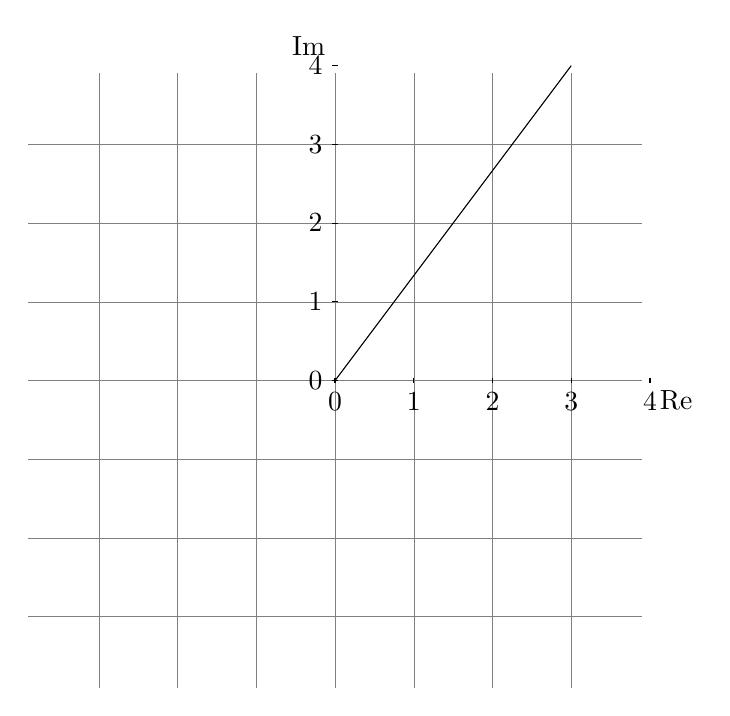
\begin{tikzpicture}
                \draw[step = 1cm, gray, very thin] (-3.9,-3.9) grid (3.9,3.9);
                \draw (0, 0) -> (3, 4);
                \foreach \x in {0,1,2,3,4}
                        \draw (\x cm,1pt) -- (\x cm,-1pt) node[anchor=north] {$\x$};
                \foreach \y in {0,1,2,3,4}
                        \draw (1pt,\y cm) -- (-1pt,\y cm) node[anchor=east] {$\y$};
                \draw (4,0) node[anchor=north west] {Re};
                \draw (0,4) node[anchor=south east] {Im};
        \end{tikzpicture}
\end{figure}


\begin{defn}[Modulus]
        The modulus of $z = x + iy \in \C$ is denoted by $|Z|$ and is equal to $|z| = \sqrt{x^2+y^2}$.
\end{defn}



\begin{defn}[Polar Form]
        For all $z \in \C$, there exists $\arg(z) \in \R$ so that $0 \leq \arg(z) < 2\pi$ and $$z = |z|(\cos(\arg(z)) + i\sin(\arg(z))) = |z|e^{i\arg(z)}$$
\end{defn}





\subsection{Theorems}

\begin{lem}[47]
        $\C$ is a field under addition and multiplication.
\end{lem}


\begin{lem}[48]
        For all $z \in \C$, $z\overline{z} \in \R$, $z\overline{z} \geq 0$ an $|z| = \sqrt{z\overline{z}}$
\end{lem}


\begin{lem}[49]
        Let $z \in \C$
        \begin{enumerate}
                \item The additive inverse of $z$ is $-z \in \C$
                \item If $z \neq 0$, then the multiplicative inverse of $z$ is $\frac{1}{z} = \frac{\overline{z}}{|z|^2} \in \C$
        \end{enumerate}
\end{lem}



\begin{lem}[50 Triangle Inequality]
        For all $z,w \in \C$, $|z+w| \leq |z| + |w|$. Moreover, $|z+w| = |z| + |w|$ $\iff$ there exists $r \in \R$, $r \geq 0$, so that $w =rz$.
\end{lem}



\begin{lem}[51]
        If $z = r_1e^{i\theta_1}$ and $w = r_2e^{i\theta_2}$, then $zw = r_1r_2e^{i(\theta_1+\theta_2)}$.
\end{lem}


\clearpage


\section{Fundamental Theorem of Algebra}


\subsection{Definitions}


\begin{defn}[Polynomial Ring over a Field]
        Let F be a field. The ring of polynomials with coefficients in F is the set $$F[x] = \{a_0 + a_1x+...+a_nx^n:n\in \N, a_i \in F,\forall 0 \leq i \leq n\}$$ which is the set of polynomials with coefficients in F.
\end{defn}


\begin{defn}[Degree]
        Let $f(x) \in F[x]$. The degree of $f$ is the largest integer $n \in \Z$ so that $a_n \neq 0$ in the expansion of $f$: $$deg(a_0+a_1x+...+a_nx^n) = n$$
\end{defn}



\begin{defn}[Rational Functions]
        The rational functions with coefficients in F are $$F(x) = \left\{\frac{p(x)}{q(x)}:p(x),q(x) \in F[x], q(x) \neq 0\right\}$$
\end{defn}



\begin{defn}[Factors]
        Let $p(x),q(x),m(x) \in F[x]$. If $p(x) = q(x)m(x)$, then $q(x)$ is a factor of $p(x)$ ($q(x) \neq 0$).
\end{defn}


\begin{defn}[Algebraically Closed]
        A field F is algebraically closed $\iff$ for all $f \in F[x]$ if $\deg(f) \geq 1$, then f has a root in F.
\end{defn}


\begin{defn}[Gaussian Integers]
        We define the Gaussian integers as the set $$\Z[i] = \{a + ib: a,b \in \Z\}$$
\end{defn}





\subsection{Theorems}


\begin{thm*}[Quotient Remainder Theorem for F[x]]
        For any polynomials $p(x),q(x) \in F[x]$ if $\deg(q) \leq \deg(p)$ and $q(x) \neq 0$, then there exist $m(x),r(x) \in F[x]$ so that $$\frac{p(x)}{q(x)} = m(x) + \frac{r(x)}{q(x)}$$ and $0 \leq \deg(r) < \deg(p)$
\end{thm*}



\begin{lem}[52]
        Let $f(x) \in F[x]$. For all $\alpha \in F$, $\alpha$ is a root of $f(x)$ if and only if $x-\alpha$ is a factor of $f(x)$.
\end{lem}



\begin{thm*}[Fundamental Theorem of Algebra]
        $\C$ is algebraically closed
\end{thm*}



\begin{cor}[53]
        Every nonconstant polynomial $f(x) \in \C[x]$ can be factored completely into a product of linear terms. That is, for all $f(x) \in \C[x]$, if $\deg(f) = n \geq 1$, there exist $k,\alpha_1,...,\alpha_n \in \C$ so that $$f(x) = k(x - \alpha_1)...(x - \alpha_n)$$
\end{cor}


\begin{lem}[54]
        For any $z,w \in \Z[i]$, $-z,\overline{z},z+w,zw \in \Z[i]$.
\end{lem}









%------------- End ----------------

\end{document}


